\chapter{Практические задания}

\begin{enumerate}[wide=0pt]
\item \textit{Представить следующие списки в виде списочных ячеек:}
\begin{enumerate}[label=\arabic*)]
	\item \lstinline {'(open close halph)}
	\item \lstinline {'((open1)(close2)(halph3))}
	\item \lstinline {'((one) for all (and (me (for you))))}
	\item \lstinline {'((TOOL) (call))}
	\item \lstinline {'((TOOL1)((call2))((shell)))}
	\item  {'(((TOOL) (call)) ((shell)))}
\end{enumerate}


\begin{figure}[ht!]
	\centering
	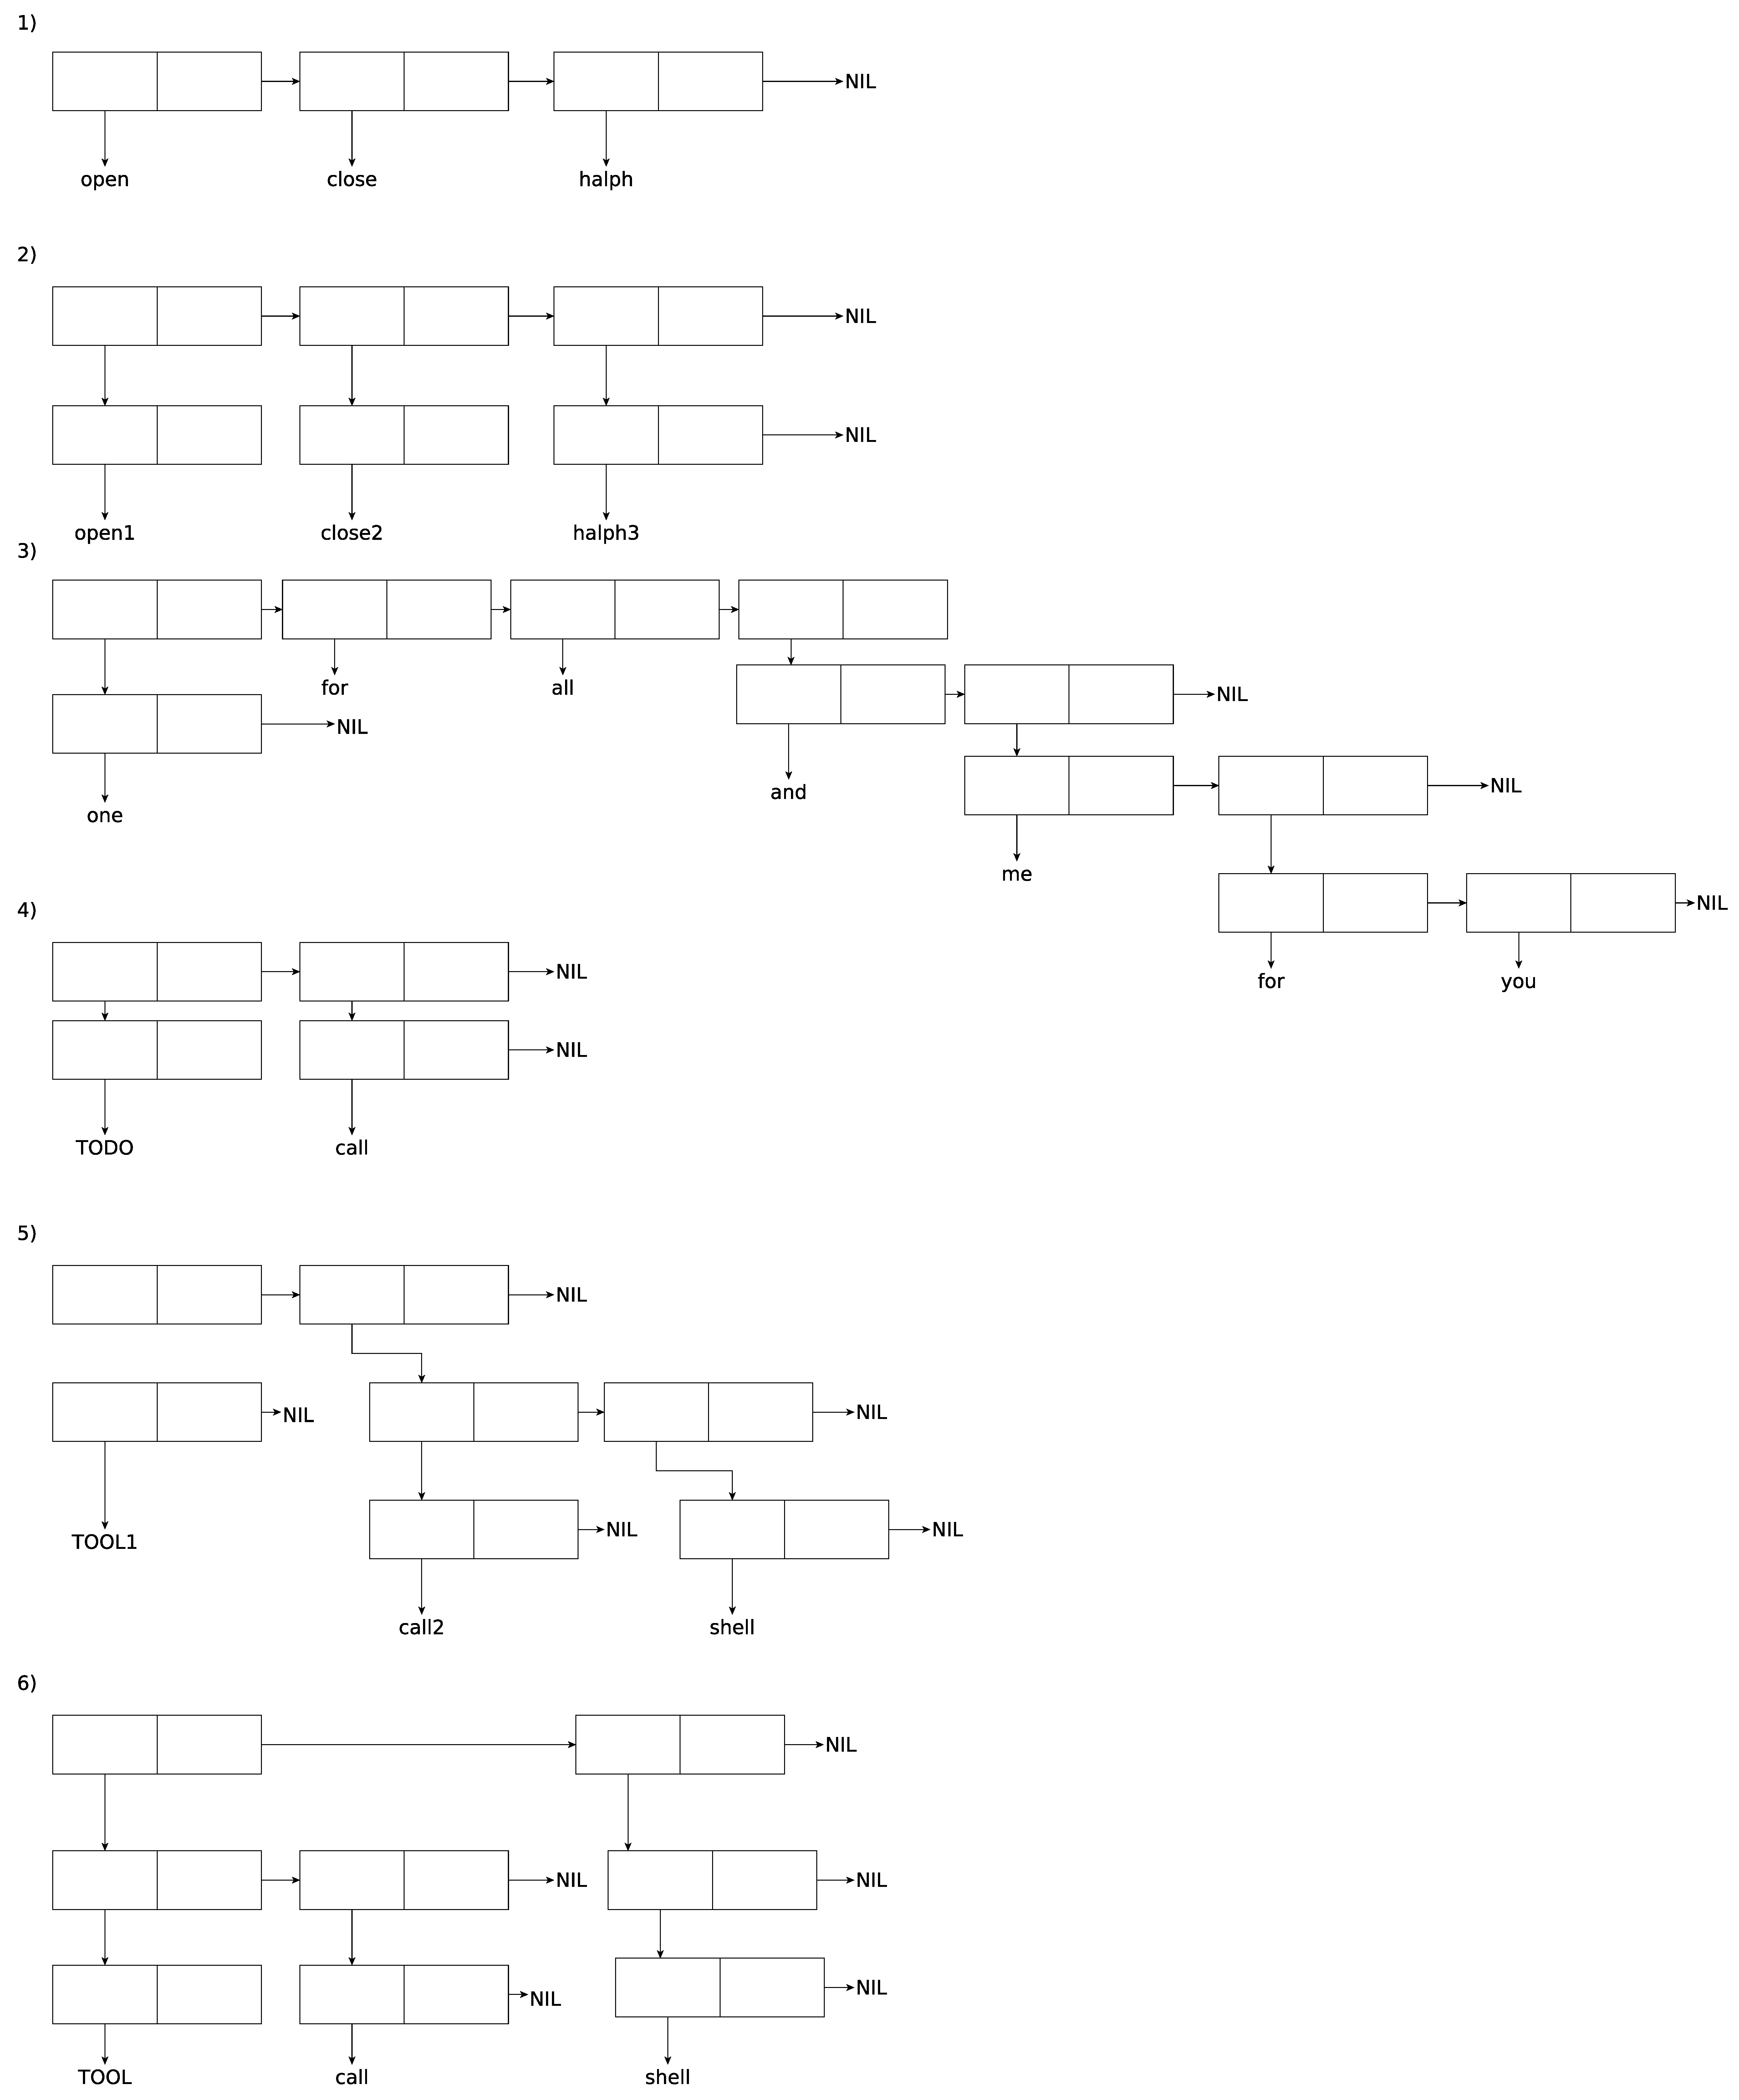
\includegraphics[width=1\linewidth]{assets/task1/1.pdf}
	\caption{Списочные ячейки. Задание 1}
\end{figure}
\FloatBarrier



\item  \textit{Используя только функции} \texttt{CAR} и \texttt{CDR} \textit{написать выражения, возвращающие:}
\begin{tasks}[label=\arabic*), item-indent=3pt, after-item-skip=1pt](3)
	\task второй; \task третий; \task четвертый элементы \\ заданного списка.
\end{tasks}
Решения:
\begin{lstlisting}
(car (cdr '(a b c d)))
(car (cdr (cdr '(a b c d))))
(car (cdr (cdr (cdr '(a b c d)))))
\end{lstlisting}
\item \textit{Что будет в результате вычисления выражений?}
\begin{tasks}[label=\arabic*), item-indent=3pt, after-item-skip=1pt, column-sep=20pt](2)
	\task \lstinline{(caadr '((blue cube) (red pyramid)))}
	\task \lstinline{(cdar '((abc)(def)(ghi)))}
	\task \lstinline{(cadr '((abc)(def)(ghi)))}
	\task \lstinline{(caddr '((abc)(def)(ghi)))}
\end{tasks}

Решения:
\begin{tasks}[label=\arabic*), item-indent=3pt, after-item-skip=1pt, column-sep=20pt](2)
	\task \lstinline{RED}
	\task \lstinline{Nil}
	\task \lstinline{(DEF)}
	\task \lstinline{(GHI)}
\end{tasks}
\item Напишите результат выражений и объясните как он получен:
\begin{enumerate}[label=\arabic*)]
	\item \lstinline{(list 'Fred 'and 'Wilma)}
	\item \lstinline{(list 'Fred '(and Wilma))}
	\item \lstinline{(cons Nil Nil)}
	\item \lstinline{(cons T Nil)}
	\item \lstinline{(cons Nil T)}
	\item \lstinline{(list Nil)}
	\item \lstinline{(cons '(T) Nil)}
	\item \lstinline{(list '(one two) '(free temp))}
	\item \lstinline{(cons 'Fred '(and Wilma))}
	\item \lstinline{(cons 'Fred '(Wilma))}
	\item \lstinline{(list Nil Nil)}
	\item \lstinline{(list T Nil)}
	\item \lstinline{(list Nil T)}
	\item \lstinline{(cons T (list Nil))}
	\item \lstinline{(list '(T) Nil)}
	\item \lstinline{(cons '(one two) '(free temp))}
\end{enumerate}
Решения:
\begin{enumerate}[label=\arabic*)]
	\item \lstinline{(FRED AND WILMA)}
	\item \lstinline{(FRED (AND WILMA))}
	\item \lstinline{(Nil)}
	\item \lstinline{(T)}
	\item \lstinline{(NIL.T)}
	\item \lstinline{(NIL)}
	\item \lstinline{((T))}
	\item \lstinline{((ONE TWO) (FREE TEMP))}
	\item \lstinline{(FRED AND WILMA)}
	\item \lstinline{(FRED WILMA)}
	\item \lstinline{(NIL NIL)}
	\item \lstinline{(T Nil)}
	\item \lstinline{(NIL T)}
	\item \lstinline{(T NIL)}
	\item \lstinline{((T) Nil)}
	\item \lstinline{((ONE TWO) FREE TEMP)}
\end{enumerate}
\item \textit{Написать лямбда-выражение и соответствующую функцию:}
\begin{tasks}[label=\arabic*), item-indent=3pt, label-offset=10pt, after-item-skip=1pt](1)
	\task Написать функцию \lstinline{f(ar1 ar2 ar3 ar4)}, возвращающую \lstinline{((ar1 ar2) (ar3 ar4))}.
	\task Написать функцию \lstinline{f(ar1 ar2)}, возвращающую \lstinline{((ar1)(ar2))}.
	\task Написать функцию \lstinline{f(ar1)}, возвращающую \lstinline{((ar1))}
	\task[~] Представить результаты в виде списочных ячеек.
\end{tasks}
Решения.
\begin{enumerate}[label=\arabic*.,wide=0pt]
\item Функция:
\begin{lstlisting}
(defun f(ar1 ar2 ar3 ar4)(cons (list ar1 ar2) (list (list ar3 ar4))))
\end{lstlisting}
Лямбда-выражение:
\begin{lstlisting}
(lambda (ar1 ar2 ar3 ar4)(cons (list ar1 ar2) (list (list ar3 ar4))))
\end{lstlisting}
\item  Функция:
\begin{lstlisting}
(defun f(ar1 ar2)(list(cons ar1 nil)(cons ar2 nil)))
\end{lstlisting}
Лямбда-выражение:
\begin{lstlisting}
(lambda (ar1 ar2)(list(cons ar1 nil)(cons ar2 nil)))
\end{lstlisting}
\item  Функция:
\begin{lstlisting}
(defun f(ar1)(list (cons ar1 nil)))
\end{lstlisting}
Лямбда-выражение:
\begin{lstlisting}
(lambda (ar1)(list (cons ar1 nil)))
\end{lstlisting}
\end{enumerate}


\begin{figure}[ht!]
	\centering
	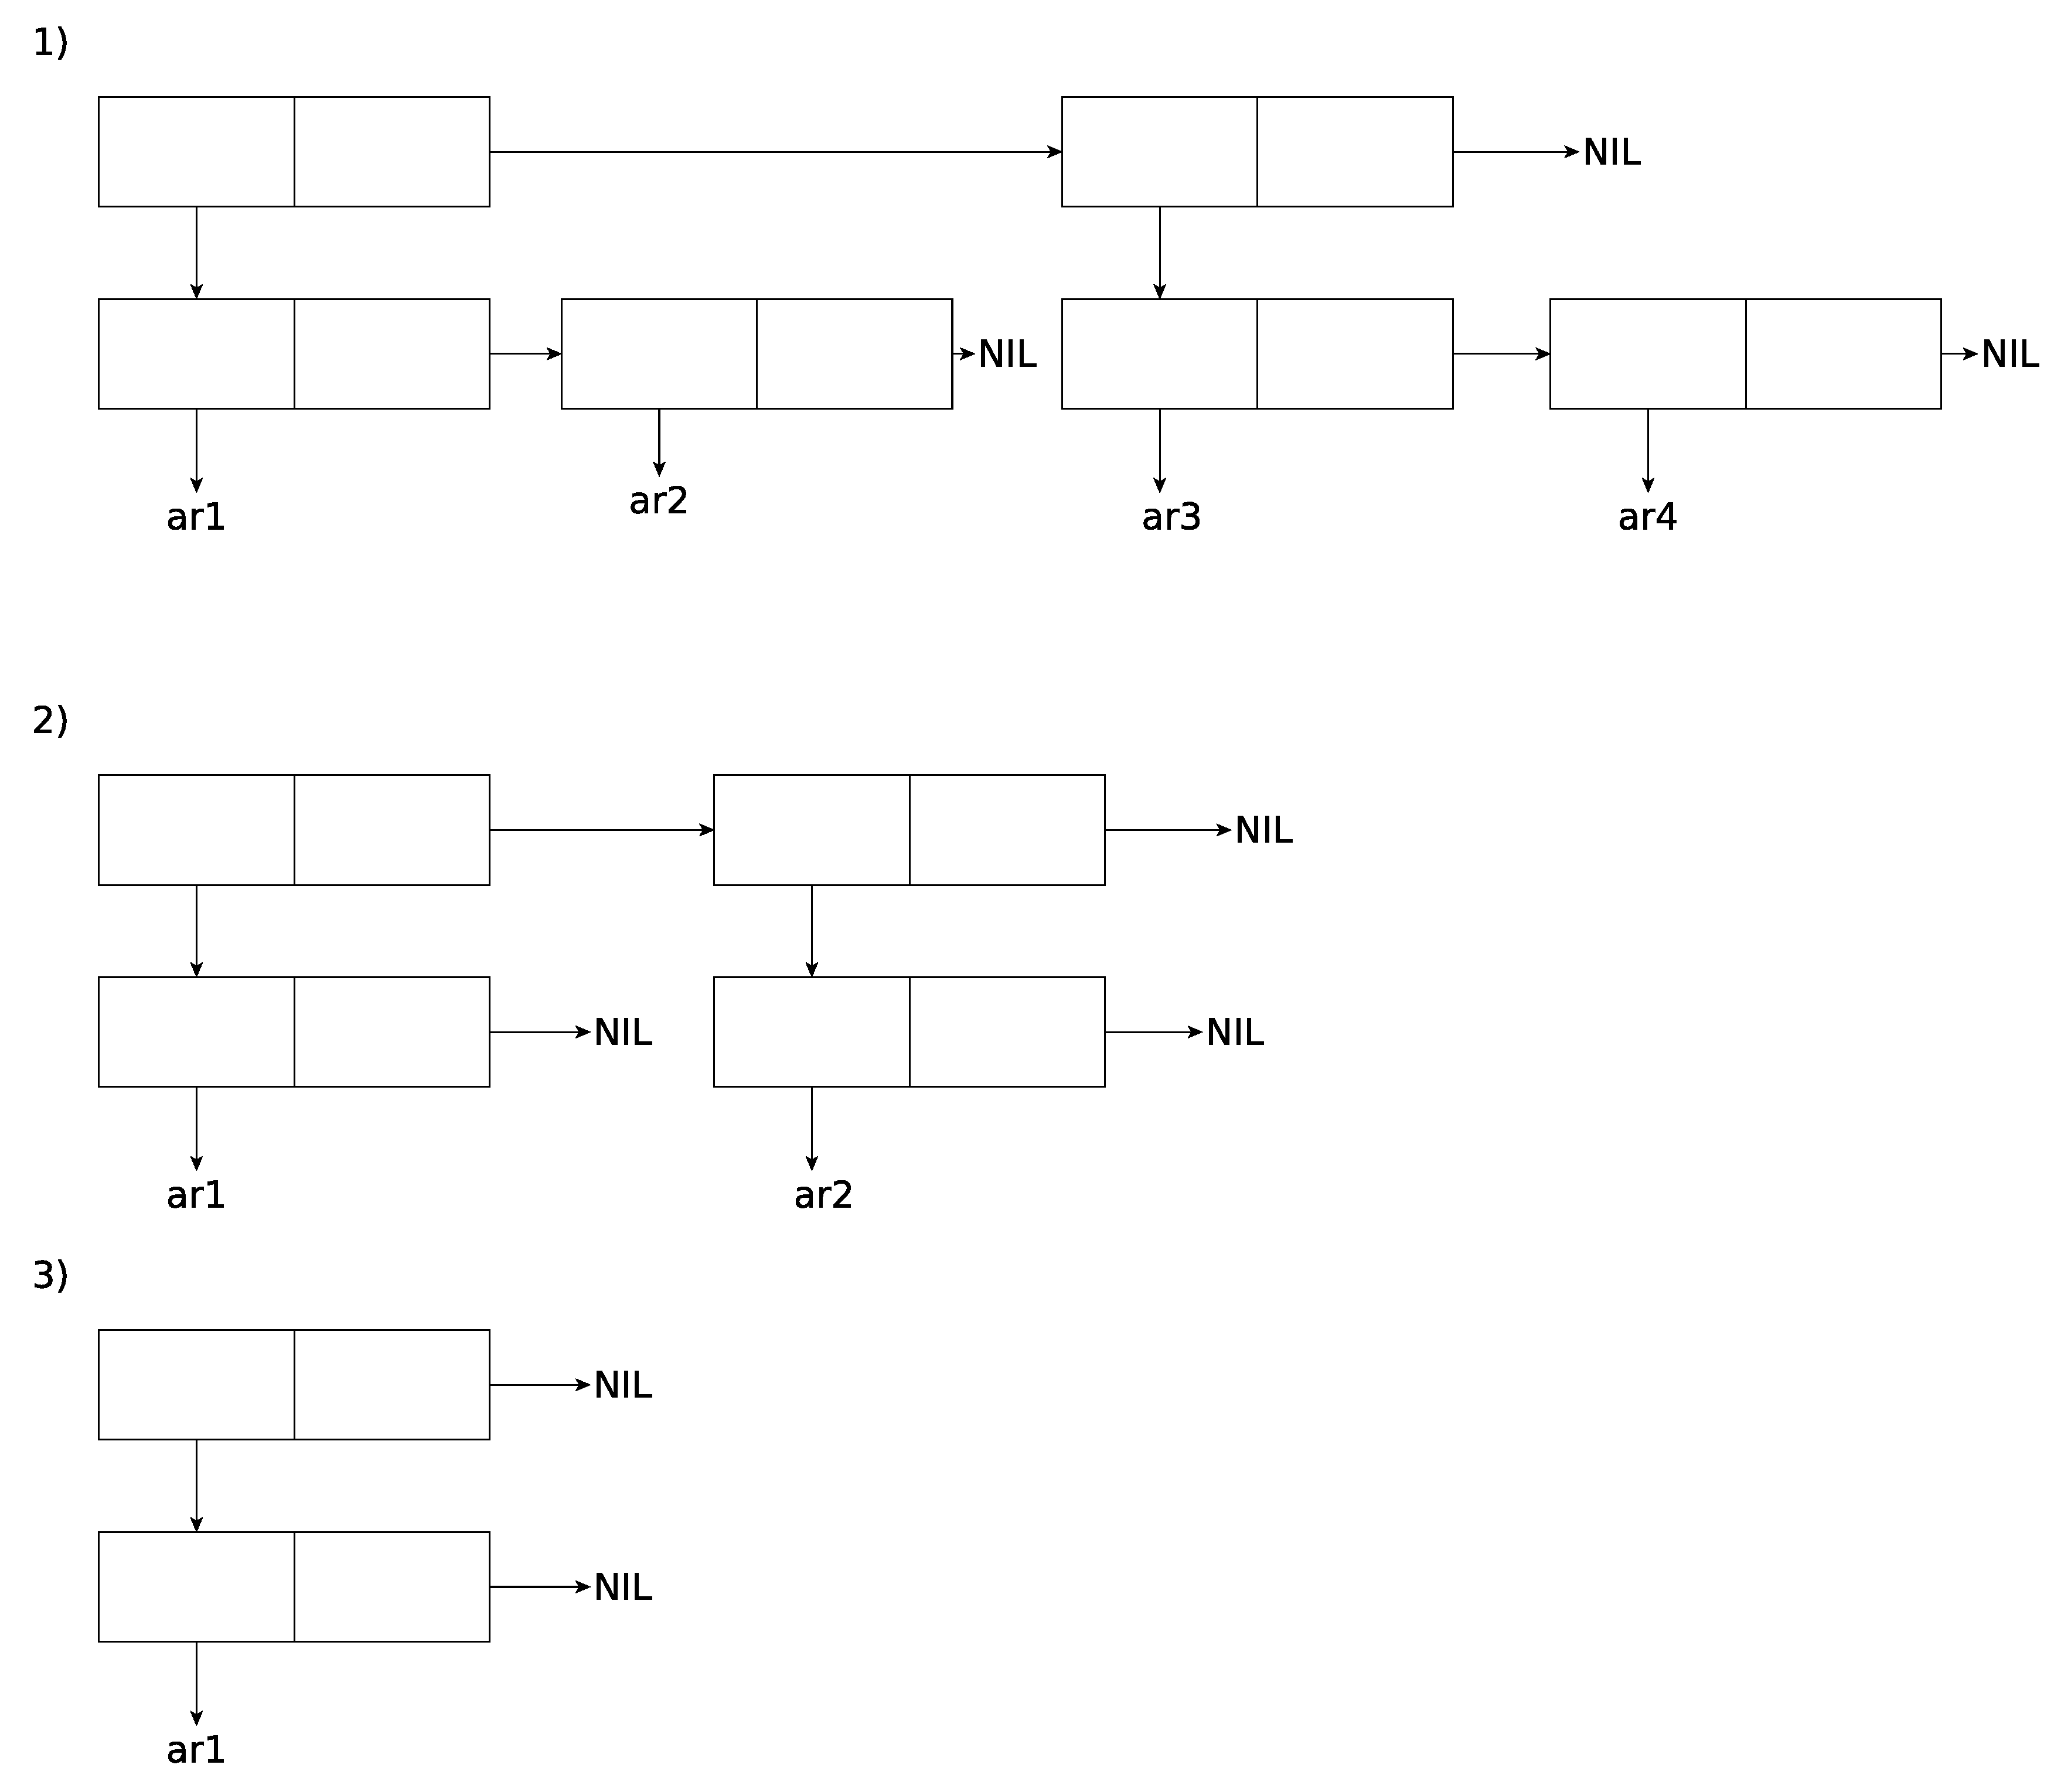
\includegraphics[width=0.9\linewidth]{assets/task1/2.pdf}
	\caption{Списочные ячейки. Задание 2}
\end{figure}
\FloatBarrier

\end{enumerate}